\chapter{Double-b tagger}
\label{ch:xbb}

\par This chapter introduces a new tagger to reconstruct boosted Higgs bosons. Section~\ref{sec:intro} gives a brief overview of this ``Xbb'' tagger. 
Monte Carlo simulation samples used for training the tagger are summarized in Section~\ref{sec:mc}.
The algorithm is introduced in Section~\ref{sec:algo}. The neural network architecture is described in Section~\ref{sec:dnn}. 
Section~\ref{sec:per} shows the performance of the tagger, which includes the signal efficiency and background mistag rate measurement.

\section{Introduction}
\label{sec:intro}

\par For a Higgs boson with \pt~above about 250 GeV, the two b quark jets merge into a single jet for a jet cone size of R = 1 ($\Delta R = \frac{2m}{p_T}$) and Higgs boson reconstruction can exploit this topology. The decaying object is reconstructed within a large-radius jet. 
The previous chapter showed studies that explored $H\rightarrow b\bar{b}$ tagging algorithms using ghost-associated subjets, 
but the performance can be further optimized using both the substructure information of the large-radius jet and the track and vertex information related to the b hadron lifetime. 
\par The approach presented here utilizes both the jet substructure and the low-level b-tagging information from the bb pair within the same large-radius jet.

\par A universal boosted Xbb tagger is built by avoiding a strong performance dependence on the large-radius jet \pt~and mass. As a result, 
the tagger can be used in many different topologies and kinematical regimes, such as searches for the Higgs boson in ttH, VH and VBF production modes, 
resonant HH and VH production, t' and b' in the tH and bH final states. The boosted Higgs tagger is also essential for this thesis - a search for a for boosted Higgs boson produced in association with dark matter. 
In principle, the algorithm should also be able to identify $Z\rightarrow b\bar{b}$, as well as any hypothetical particle decaying into a $b\bar{b}$ pair with a mass close to the W/Z/H boson mass.

\section{Monte Carlo Simulation Samples}
\label{sec:mc}

\par A sample of background jets initiated by light quarks and gluons is derived from a multijet process simulated using PYTHIA8~\cite{Sjostrand:2007gs} with the NNPDF2.3 leading order (LO) parton distribution 
function (PDF) set~\cite{Ball:2012cx} and the A14~\cite{ATL-PHYS-PUB-2014-021} tune for underlying event parameterisations. 
Jets from this sample are referred to as QCD jets. Fully hadronic top quark pair events are used for jets originating from hadronic top quark decays (top jets) and are generated 
using POWHEG~\cite{Frixione:2007vw,Nason:2004rx} interfaced to PYTHIA6~\cite{Sjostrand:2006za} with the PERUGIA 2012~\cite{Skands:2010ak} underlying event tune parameter set 
and the four flavor scheme of the CT10 PDF set ~\cite{Gao:2013xoa}.
\par For the boosted Higgs jets, a sample of high \pt~Higgs bosons is obtained from the BSM physics simulation of a Randall-Sundrum graviton decaying to a pair of Higgs bosons with both Higgs bosons 
subsequently decaying to $b\bar{b}$ pairs ($g\rightarrow HH \rightarrow b\bar{b}b\bar{b}$)~\cite{Randall:1999ee}. This process is generated using MadGraph5~\cite{Alwall:2014hca} 
interfaced with PYTHIA8 and with the ATLAS A14 tune, and the NNPDF2.3 LO PDF set. The mass splitting between the massive graviton and the Higgs boson provides a boost proportional to the mass of the graviton. 
Therefore, signal samples have been generated with graviton masses between 300 GeV and 6000 GeV to fully populate the kinematic region of interest. 
The signal samples of various masses are merged and both top and signal samples are reweighted on a jet-by-jet basis such that the large-radius calorimeter jet kinematics in signal matches that of the QCD jet sample in \pt~and $\eta$. 
This reweighting is intended to mitigate the effects of any difference in kinematics present between the unweighted samples. 
EvtGen~\cite{Lange:2001uf} is used to model the decays of b- and c-flavoured hadrons.
\par The Monte Carlo samples are processed through the full ATLAS detector simulation~\cite{Aad:2010ah} with the tool Geant4~\cite{Agostinelli:2002hh}, and reconstructed using the standard ATLAS reconstruction software. Simulated minimum-bias events are added to the events to match the pile-up distribution in data. 

\section{Double-b tagger algorithm}
\label{sec:algo}

\par As shown in the Chapter~\ref{ch:objects}, the previous approach requires matching the large-radius jet which are used to reconstruct Higgs boson with two track jets.
\par The standard single-b tagging algorithm is applied to the track jets to identify subjets from single b quarks. With its focus on individual subjets, the subjet single-b tagging does not make use of the global properties of the large-radius jets which contain two b hadrons. Even though the algorithm performs well in the high purity regime, relying heavily on the reconstruction of secondary vertices associated with the subjets, at high \pt, the subjets start to overlap and cause the standard single b tagging techniques to break down due to double-counting of tracks and secondary vertices when computing the subjet single b-tagging discriminants. 
\par To discriminate $b\bar{b}$ pairs originated from Higgs bosons from QCD jets initiated by single partons, a boosted Higgs tagger with large signal-to-background ratio is built using a deep neural network (DNN) which fully exploits the presence of two b quarks inside a large radius jet and their topology in relation to the jet substructure. 

\subsection{Input features}

\par The inputs fed into the neural networks are both features of the subjets declustered from the large-radius jet and features that describes the correlation between the subjets.
\par For each subjet,
\begin{itemize}
    \item To reconstruct b hadron decay vertices, we apply the Inclusive secondary vertex (SV1) algorithm which identifies secondary vertices independently of the jet clustering.
    \item We reconstruct the decay chains of the two b hadrons by associating reconstructed secondary vertices to the subjet axis via JetFitter.
    \item We use the output scores of two algorithm, IP3D/IP2D (using likelihood-ratio method) and RNNIP (using recurrent neural networks) which process charged particle tracks associated to jets without reliance on secondary 
    vertex finding to augment secondary-vertex based taggers. 
\end{itemize}

\par Similarly to the single-b tagger (MV2c10), the scores from these low-level taggers are all fed into the neural network to complement each other's performance.

\par All input features constructed within each subjet that are used for the training are listed in Table~\ref{tab:input}.

\begin{table}[tbh]
    \centering
    \begin{tabular}{|l|l|}
        \hline
        Low-level Algorithm & Algorithm Outputs (Training inputs) \\
        \hline
        \hline
        IP2D(IP3D) & \speciallcell{IP2D\_pu, IP2D\_pb, IP2\_pc,\\ IP3D\_pu, IP3D\_pb, IP3D\_pc} \\
        \hline
        RNNIP & \speciallcell{RNNIP\_pu, RNNIP\_pb,\\ RNNIP\_pc, RNNIP\_tau} \\
        \hline
        SV1 & \speciallcell{sv1\_ntkv, sv1\_n2t, sv1\_mass,\\ sv1\_efrc, sv1\_dR, SV1\_dstToMatLay,\\ SV1\_Lxy, SV1\_L3d, sv1\_sig3} \\
        \hline
        JetFitter & \speciallcell{jf\_n2tv, jf\_ntrkv, jf\_ntvx,\\ jf\_ntvx1t, jf\_mass,\\ jf\_efrc, jf\_dR, jf\_sig3,\\ JetFitter\_deltaphi, JetFitter\_deltaeta} \\
        \hline
    \end{tabular}
    \caption{Input features used for training double-b tagger.}
    \label{tab:input}
\end{table}

\par In addition, the following features are used to describe the correlations:

\begin{itemize}
    \item Subjet kinematic variables: \pt~and $\eta$.
    \item Subjet angular variables: $d R$, $d\eta$, $d\phi$ with respect to the parent large-radius jet.
    \item Event-based variables: \pt~imbalance between subjets which indicates the ratio of each subjet momentum to the total momentum.
\end{itemize}

\section{Neural network architecture}
\label{sec:dnn}

\par A feed-forward, fully connected neural network~\cite{hopfield1982neural} with 6 hidden layers, 164 input features and 2 or 3 outputs is designed. While a batch normalization layer is applied at the input layer, each hidden layer of the neural network is built from the following components:

\begin{itemize}
    \item Dense layer: defined as a linear combination of all outputs from the previous layer.
    \item Batch normalization layer: to transform the inputs to zero-mean and unit-variance. ~\cite{DBLP:journals/corr/IoffeS15}
    \item Dropout layer: an operation that drops a fixed fraction of randomly chosen nodes, used as a regularization handle. The dropout rate is one of the optimized hyperparameters of the neural network~\cite{JMLR:v15:srivastava14a}.
    \item Activation unit: we use the Rectified Linear Unit (ReLU)~\cite{Pich:1998xt}:	
\end{itemize}

\begin{equation}
    f(x) = \left \{ \begin{array}{rcl}0 & \mbox{for} & x $<$ 0,\\ x & \mbox{for} & x \ge 0,\end{array} \right. \label{eq:relu}
\end{equation}

\par To optimize the performance of the neural network, three hyperparameters are considered: the depth of the network architecture, the dropout rate and the learning rate. The following values are considered:

\begin{itemize}
    \item Dropout rate: 0.1, 0.2, 0.3, 0.4, 0.5;
    \item Number of hidden layers: 3, 4, 5, 6, 7;
    \item Learning rate: $10^{−1}$, $10^{−2}$, $10^{−3}$, $10^{−4}$, $10^{−5}$.
\end{itemize}

\par Out of 125 grid points in the hyperparameter space, 50 combinations are randomly sampled. From all the configurations with comparable performance, the network with the smallest number of trainable parameters was chosen. 
\par We start with learning rate = 0.1 and uses an adaptive learning rate which means decreasing the learning rate by a factor of three once the performance of the model plateaus. Also, early stopping~\cite{Yao07onearly} which allows 20 training epochs and stops training once the model performance stops improving on a hold out validation dataset are applied as regularization. 

\section{Signal efficiency and Background mistag rate measurement}
\label{sec:per}

\par Both signal efficiency and background mistag rate of the double-b tagger are evaluated with the testing samples which are independent of the training samples.

\par Performances of the following taggers are evaluated: DL-tag refers to a bi-class discriminator that distinguishes QCD from Higgs with input features from each subjet, and subjet correlation. 
XbbScore is a multiclass discriminator (QCD, Higgs, Top) which also includes other large-radius jet substructure features in the input features. 
The baseline boosted Hbb tagger, which identifies a large-radius jet with two ghost-associated track jets (2-tag) or one b-tagged track jet (1-tag leading jet), is used for comparison.
\par The performance can be expressed in terms of its receiver operator characteristic (ROC) plot, which shows the change of background rejection as a function of the Higgs boson tagging efficiency. Fig.~\ref{fig:xbb_roc} (left) compares double-b taggers with the baseline boosted Higgs tagger while the right plot compares XbbScore which trains Hbb against QCD and top jet with a top tagger built on a neural network and the jet substructure variable $\tau_{32}$.
\par In general, the double-b tagger outperforms the baseline boosted Hbb and top tagger. At the same signal efficiency, the mistag rate of the new method is uniformly lowered by about a factor of 2 to 5.

\begin{figure}[htbp!]
    \centering
    \includegraphics[clip, trim=0 9cm 0 0, width=1\textwidth]{chapters/c10/figures/roc}
    \caption{ROC plot: Comparison between Hbb taggers (Left) and Top taggers (Right).}
    \label{fig:xbb_roc}
\end{figure}

\par In Fig.~\ref{fig:xbb_pt}, the signal efficiencies and mistag rates for the double-b tagger as a function of large-radius jet \pt~are reported with the baseline boosted Hbb tagger for comparison.

\par The left plot shows the Higgs efficiency for a fixed 70\% working point (WP) cut as a function of large-radius jet \pt. To isolate the effect of a changing Higgs efficiency from that of the changing dijets rejection, the right plot shows a flat-efficiency 70\% WP, which means all taggers have a 70\% efficiency across \pt~and only the rejection is varying. The mistag rate is relatively flat across the \pt~range, while the signal efficiency decreases with increasing \pt, as expected from the deregradation of the tracking performance inside high \pt~jets. 
Again, double-b tagger outperforms the baseline boosted Hbb tagger.

\begin{figure}[htbp!]
    \centering
    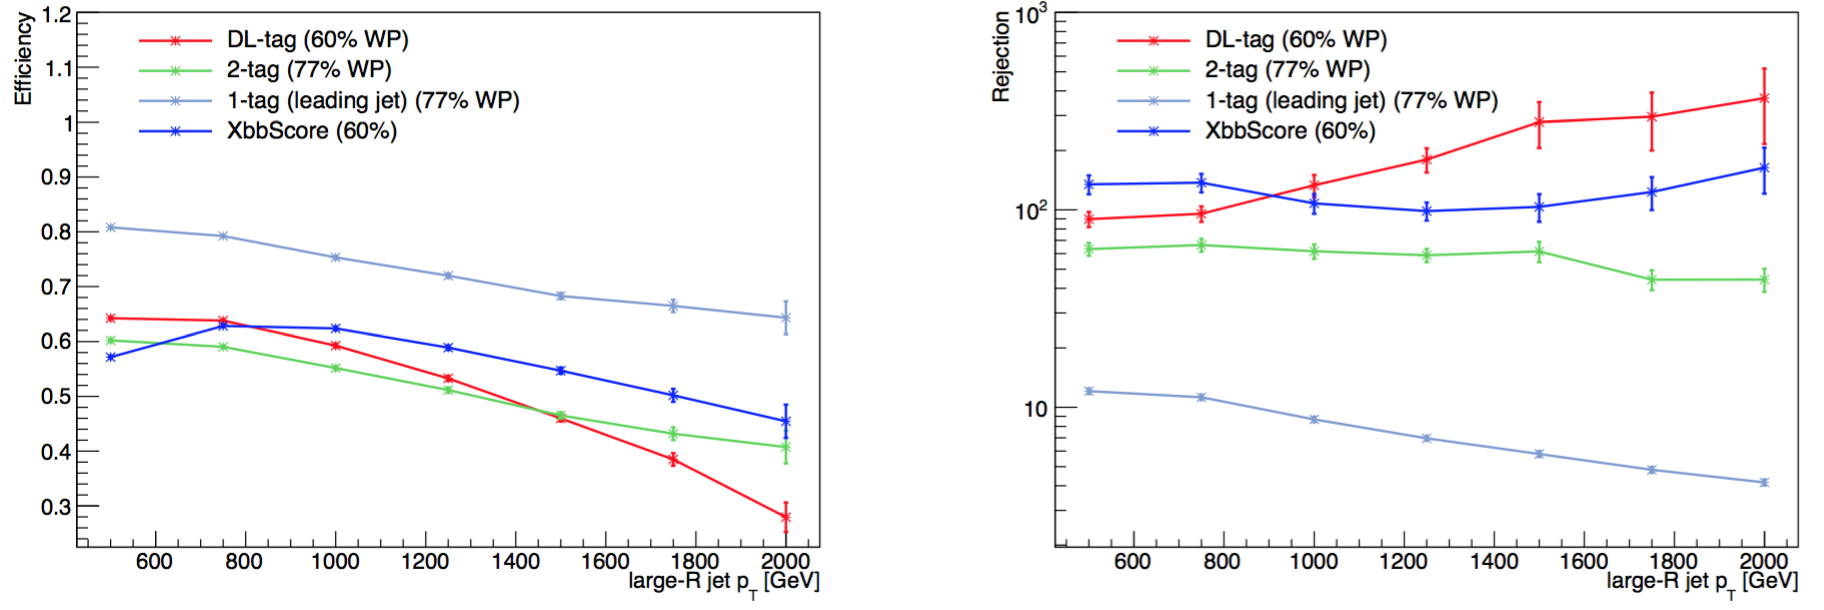
\includegraphics[clip, trim=0 0 0 0, width=1\textwidth]{chapters/c10/figures/pt}
    \caption{Higgs efficiency (left) and Background rejection (right) as a function of large-radius jet \pt}
    \label{fig:xbb_pt}
\end{figure}
